\documentclass[twoside]{article}
\setlength{\oddsidemargin}{0.25 in}
\setlength{\evensidemargin}{-0.25 in}
\setlength{\topmargin}{-0.6 in}
\setlength{\textwidth}{6.5 in}
\setlength{\textheight}{8.5 in}
\setlength{\headsep}{0.75 in}
\setlength{\parindent}{0 in}
\setlength{\parskip}{0.1 in}

\usepackage{graphicx}
\usepackage{url}

%
% The following commands sets up the lecnum (lecture number)
% counter and make various numbering schemes work relative
% to the lecture number.
%
\newcounter{lecnum}
\renewcommand{\thepage}{\thelecnum-\arabic{page}}
\renewcommand{\thesection}{\thelecnum.\arabic{section}}
\renewcommand{\theequation}{\thelecnum.\arabic{equation}}
\renewcommand{\thefigure}{\thelecnum.\arabic{figure}}
\renewcommand{\thetable}{\thelecnum.\arabic{table}}
\newcommand{\dnl}{\mbox{}\par}

%
% The following macro is used to generate the header.
%
\newcommand{\lecture}[4]{
  \pagestyle{myheadings}
  \thispagestyle{plain}
  \newpage
  \setcounter{lecnum}{#1}
  \setcounter{page}{1}
  \noindent
  \begin{center}
  \framebox{
     \vbox{\vspace{2mm}
   \hbox to 6.28in { {\bf COMPSCI~590S~~~Systems for Data Science
                       \hfill Fall 2016} }
      \vspace{4mm}
      \hbox to 6.28in { {\Large \hfill Lecture #1: #2  \hfill} }
      \vspace{2mm}
      \hbox to 6.28in { {\it Lecturer: #3 \hfill Scribe(s): #4} }
     \vspace{2mm}}
  }
  \end{center}
  \markboth{Lecture {#1}: #2}{Lecture {#1}: #2}
  \vspace*{4mm}
}

%
% Convention for citations is authors' initials followed by the year.
% For example, to cite a paper by Leighton and Maggs you would type
% \cite{LM89}, and to cite a paper by Strassen you would type \cite{S69}.
% (To avoid bibliography problems, for now we redefine the \cite command.)
%
\renewcommand{\cite}[1]{[#1]}

% \input{epsf}

%Use this command for a figure; it puts a figure in wherever you want it.
%usage: \fig{NUMBER}{FIGURE-SIZE}{CAPTION}{FILENAME}
\newcommand{\fig}[4]{
           \vspace{0.2 in}
           \setlength{\epsfxsize}{#2}
           \centerline{\epsfbox{#4}}
           \begin{center}
           Figure \thelecnum.#1:~#3
           \end{center}
   }

% Use these for theorems, lemmas, proofs, etc.
\newtheorem{theorem}{Theorem}[lecnum]
\newtheorem{lemma}[theorem]{Lemma}
\newtheorem{proposition}[theorem]{Proposition}
\newtheorem{claim}[theorem]{Claim}
\newtheorem{corollary}[theorem]{Corollary}
\newtheorem{definition}[theorem]{Definition}
\newenvironment{proof}{{\bf Proof:}}{\hfill\rule{2mm}{2mm}}

% Some useful equation alignment commands, borrowed from TeX
\makeatletter
\def\eqalign#1{\,\vcenter{\openup\jot\m@th
 \ialign{\strut\hfil$\displaystyle{##}$&$\displaystyle{{}##}$\hfil
     \crcr#1\crcr}}\,}
\def\eqalignno#1{\displ@y \tabskip\@centering
 \halign to\displaywidth{\hfil$\displaystyle{##}$\tabskip\z@skip
   &$\displaystyle{{}##}$\hfil\tabskip\@centering
   &\llap{$##$}\tabskip\z@skip\crcr
   #1\crcr}}
\def\leqalignno#1{\displ@y \tabskip\@centering
 \halign to\displaywidth{\hfil$\displaystyle{##}$\tabskip\z@skip
   &$\displaystyle{{}##}$\hfil\tabskip\@centering
   &\kern-\displaywidth\rlap{$##$}\tabskip\displaywidth\crcr
   #1\crcr}}
\makeatother

% **** IF YOU WANT TO DEFINE ADDITIONAL MACROS FOR YOURSELF, PUT THEM HERE:



% Some general latex examples and examples making use of the
% macros follow.

\begin{document}

%FILL IN THE RIGHT INFO.
%\lecture{**LECTURE-NUMBER**}{**DATE**}{**LECTURER**}{**SCRIBE**}
\lecture{14}{Bloom Filter, Distributed Shared Memory and Spark}{Emery Berger}{Namrita Pandita, Mark Saad}

\section{Bloom Filter [Used in BigTable] }
What is Bloom Filter?
\begin{itemize}
\item	tries to find if an element x is in set S
\item	has one way error meaning:
\begin{itemize}
\item	If it returns false then x definitely does not belong to S
\item	If it returns true then we don’t know! X may or may not belong to S
\end{itemize}
\end{itemize}
Why is it needed?
\begin{itemize}
\item	And most cases are expected to false and returning false is really fast and reliable.
\item	Compact representation
\begin{itemize}
\item	For a set from 0 to 15
\begin{itemize}
\item  A set of 16 bits: 0 represents that the item is not in the set, 1 is in the set. This if you know the cardinality and it’s compact
\end{itemize}
\item	Else, like if you’re doing all the names in the US
\begin{itemize}
\item 	Use hash map, or use bloom set for all Americans (first + last) name. basically a set of zeros and you OR in every new name. 
\item	examples: 
\begin{itemize}
\item	check if Mickey is in the set -> hash(“Mickey”) = 11 or “1011” in binary
\item	if current set is S = { 0000000110 } it returns false[ because all bits set in hash of “Mickey” are not set in S], therefore Mickey is not in the set
\item	check if Molly is in the set -> hash(“Molly”) = 2 or “10” in binary
\item	returns true, therefore Molly may or may not exist in the set
\end{itemize}

\item	the hash takes everybody in the set and distributes them, ideally randomly
\item	it is usually a good idea to have a big enough bloom set so that you have less collisions
\end{itemize}
\end{itemize}
\end{itemize}


\section{Distributed Shared Memory }

The idea is to partition memory [RAM] into machines in the cluster. Partitioning may be done equally or using hashing. DSM is very fine grained [has direct access to memory].
\par
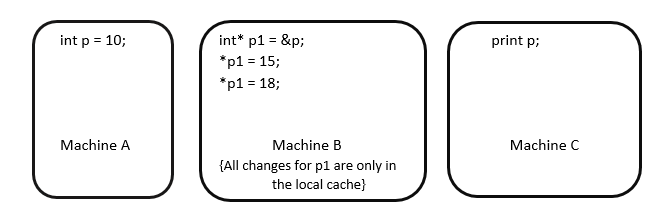
\includegraphics[scale=1]{fig-1.PNG}
\par
Issues:

\begin{itemize}
\item Cache consistency (who sees what when)
\begin{itemize}
\item	Professor Emery thinks this is never gonna work: you have memory, it’s close, it’s fast, the end
\end{itemize}
\item	Race Conditions
\item	Example: 

\begin{itemize}
\item	Cache Inconsistency: Machine B thinks p = 18, but Machine C thinks it is still 10, value in machine A is stale
\item	Race Conditions: if Reads and writes to the same memory location occur simultaneously, the results will never be deterministic.  
\end{itemize}
\end{itemize}
\section{Spark }
Spark is an API on top of RDDs:
\begin{itemize}
\item	coarse-grained: less message traffic, it means that it can work on several or all objects at the same time, instead of looping over objects to set a value. You call a method like “setAll” and it does it for you in parallel, the same for a map function. Spark has datasets and coarse-grained operators that applies to everything or several items at a time.
\item	Deterministic: you don’t have to worry about locks. [No Race Conditions]
\item	Immutable: state can’t be changed; the item is not being modified in place. it also means that caching is fine and it’s better for parallelism [No Cache Inconsistency]
\end{itemize}
Lineage: low disk bandwidth, immutable operations, can be replayed easily. Ensures Fault tolerance.
\par
RDDs are read-only in the sense that it’s write-once actions or transformations that operate on RDDs and create new RDDs
\par
Persist is a misused term, in Spark’s world it means save to memory (RAM) instead of the real meaning of persist which means write to disk 
\par If you don’t call persist, RDDs will be garbage collected
\par Spilling: RDDs can be written on disk (HDFS) if there’s no available memory.
\par Serialization translates an object to a JSON-like format to transfer it to other machines, in order to avoid collisions. Spark is de-serialized. It is faster but not so memory efficient. Serialized version is more compact and highly optimized but has slow iteration. Serialization is needed if Java objects need to be moved from one machine to another.

Narrow vs wide
\begin{itemize}
\item	Narrow is an operation that just goes from one to one on the same machine like a map operation without a shuffle 
\item	Wide is an operation like join where it has implications for lineage. Has a shuffle involved [one-to-many or many-to-many]
\end{itemize}
Spark’s Design:
\begin{itemize}
\item	Batch Analysis: focused on iteration and is coarse grained
\item	Is not interactive and write intensive transactional
\item	Spark can be stated as Scala implementation of DryadLINQ along with RDDs.
\end{itemize}
\end{document}
